\setcounter{chapter}{1}
\chapter{Neuroanatomy}
\label{sec:neuro}
%
\comment{\paragraph{Ziele:} 
\begin{itemize}
    \item uebersicht neuroanatomy
    \item struktureller aufbau nervenfaser
    \item ableitbare eigenschaften fuer modelle
\end{itemize}}
%
\section{Evolution/Introduction}
%
\section{Brain Architecture}
% 
\ac{WM},\ac{GM}.
%
\begin{figure}[!t]
\centering
\subcaptionbox{}[.28\textwidth]{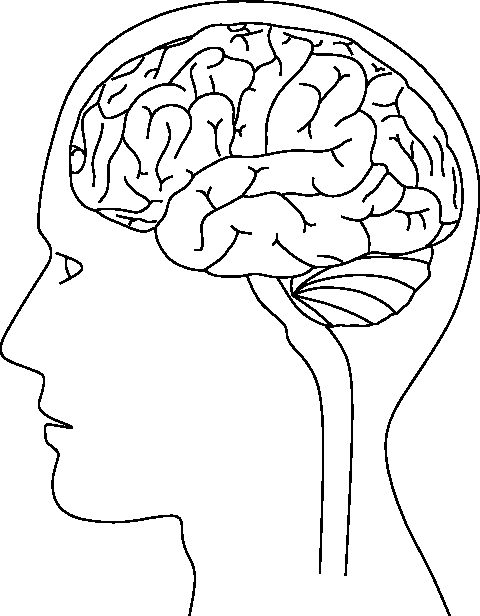
\includegraphics[height=3cm]{gfx/neuroanatomy/human-brain-profile.pdf}}
\subcaptionbox{}[.35\textwidth]{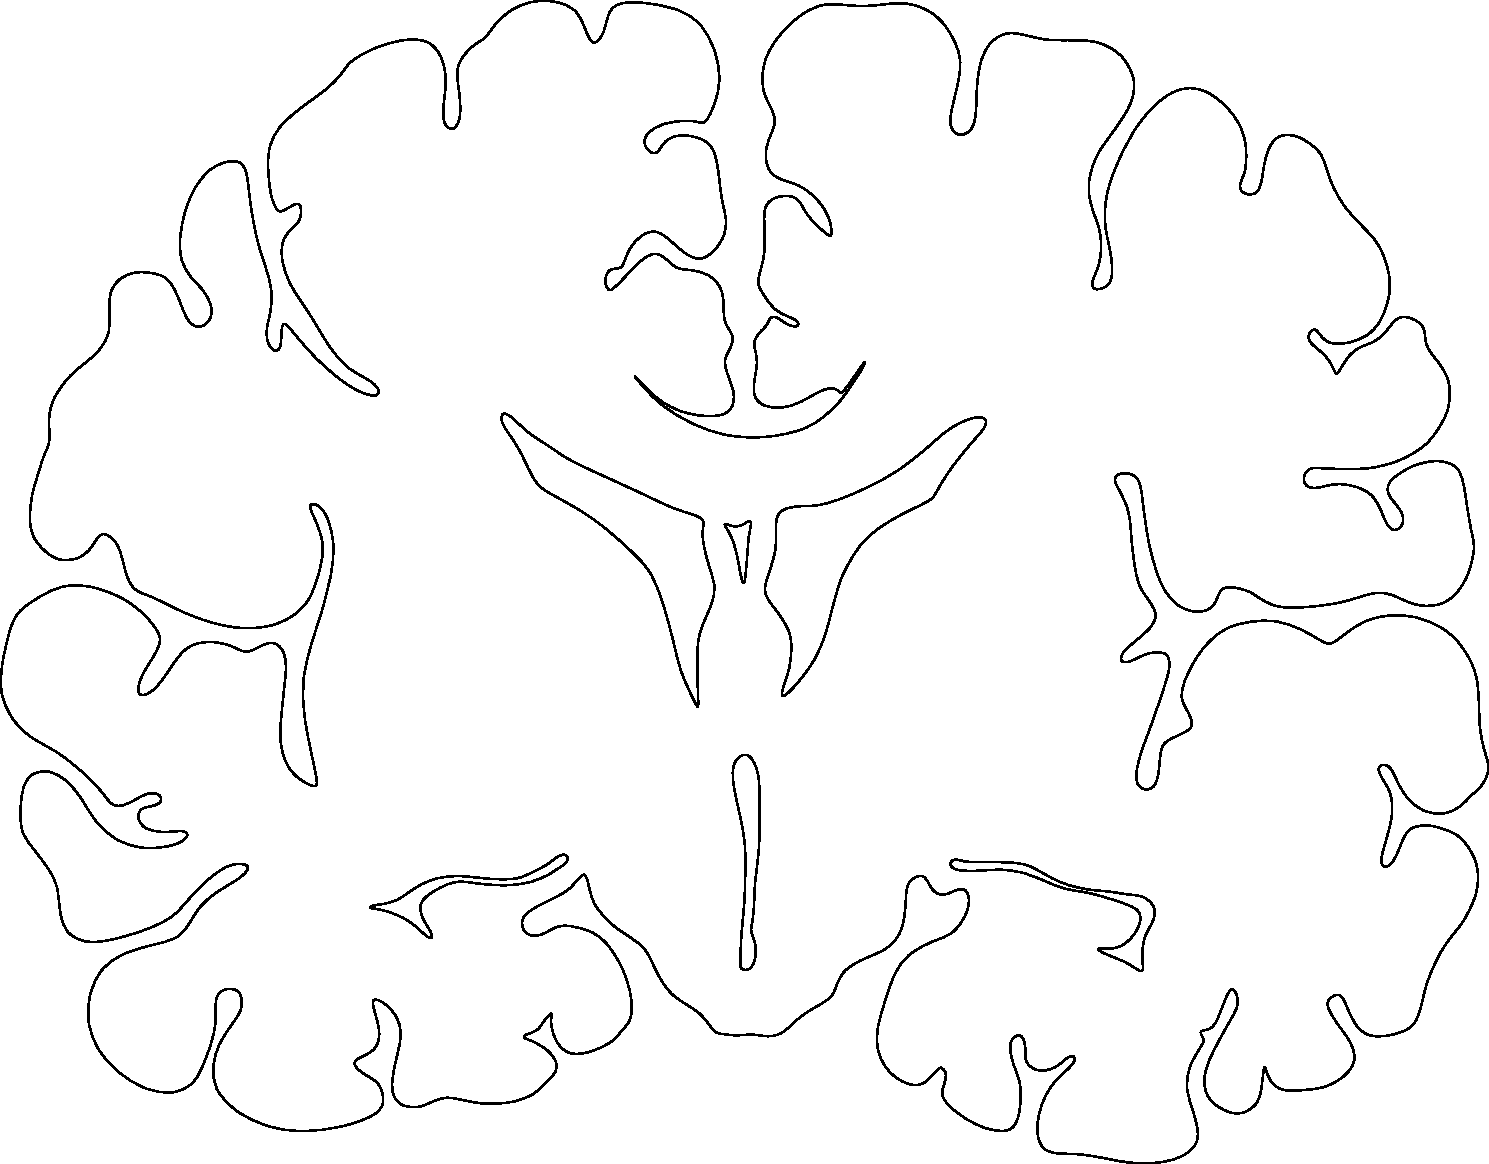
\includegraphics[height=3cm]{gfx/neuroanatomy/human-brain-section.pdf}}
\subcaptionbox{\label{fig:nerveFiber}}[.35\textwidth]{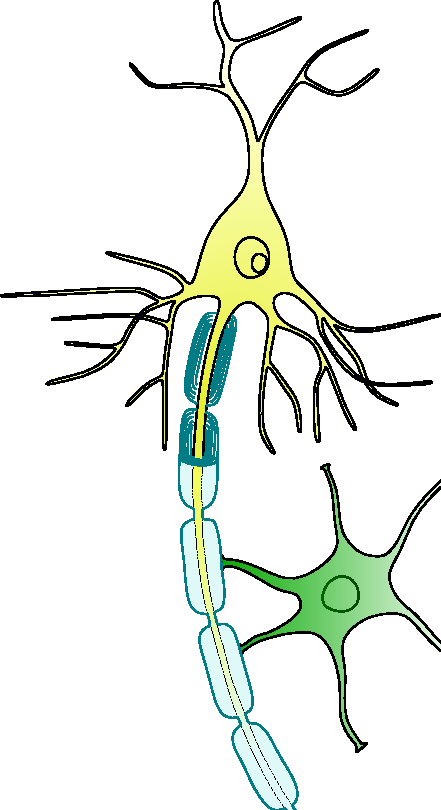
\includegraphics[height=3cm]{gfx/neuroanatomy/neuron-axon.pdf}}
\caption{(a) Illustration of human brain. (b) Illustration of a coronal human brain section. (c) Illustration of a neuron with axon and oligodendrocytes.}
\label{fig:human-brain}
\end{figure}
%
\section{Fiber Architecture} \label{sec:fiberArchitecture}
%
\section{Sectioning}
%
\begin{figure}[!t]
	\centering
    \def\tikzwidth{0.75\textwidth}
	\inputtikz{gfx/neuroanatomy/brain_sectioning}
	\caption{Illustration of sectioning.}
	\label{fig:brain_sectioning}
\end{figure}
% 
\begin{figure}[!t]
	\centering
	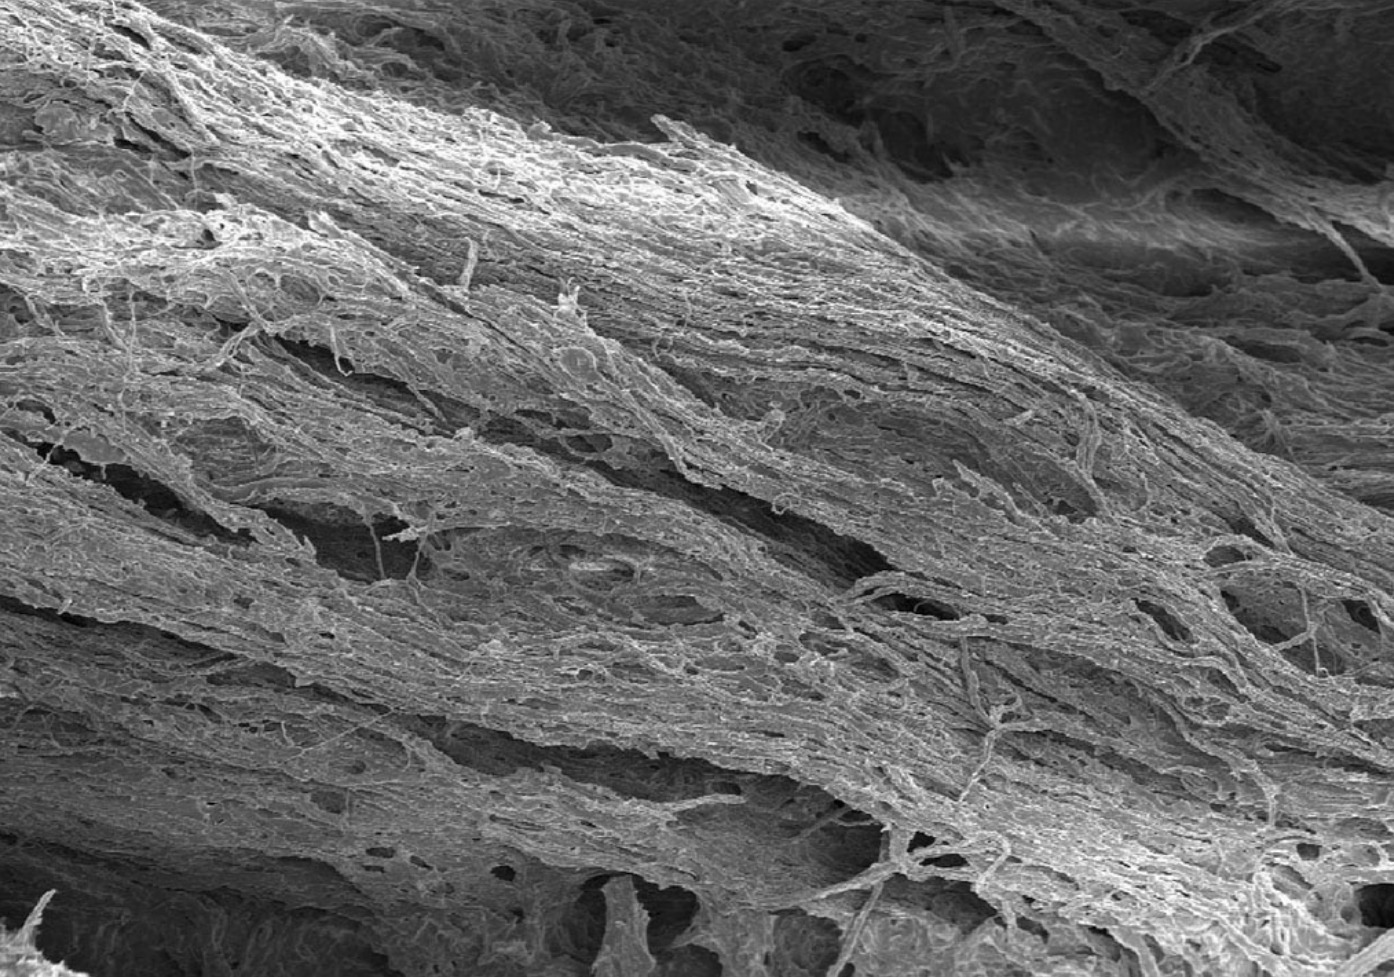
\includegraphics{gfx/neuroanatomy/human_wm_after_klinger_dissection.png}
	\caption{Electron microscopy image after klinger dissection \cite{destrieux:hal-01261930}.}
% 	\label{fig:brain_sectioning}
\end{figure}
% 
\begin{figure}[!t]
	\centering
	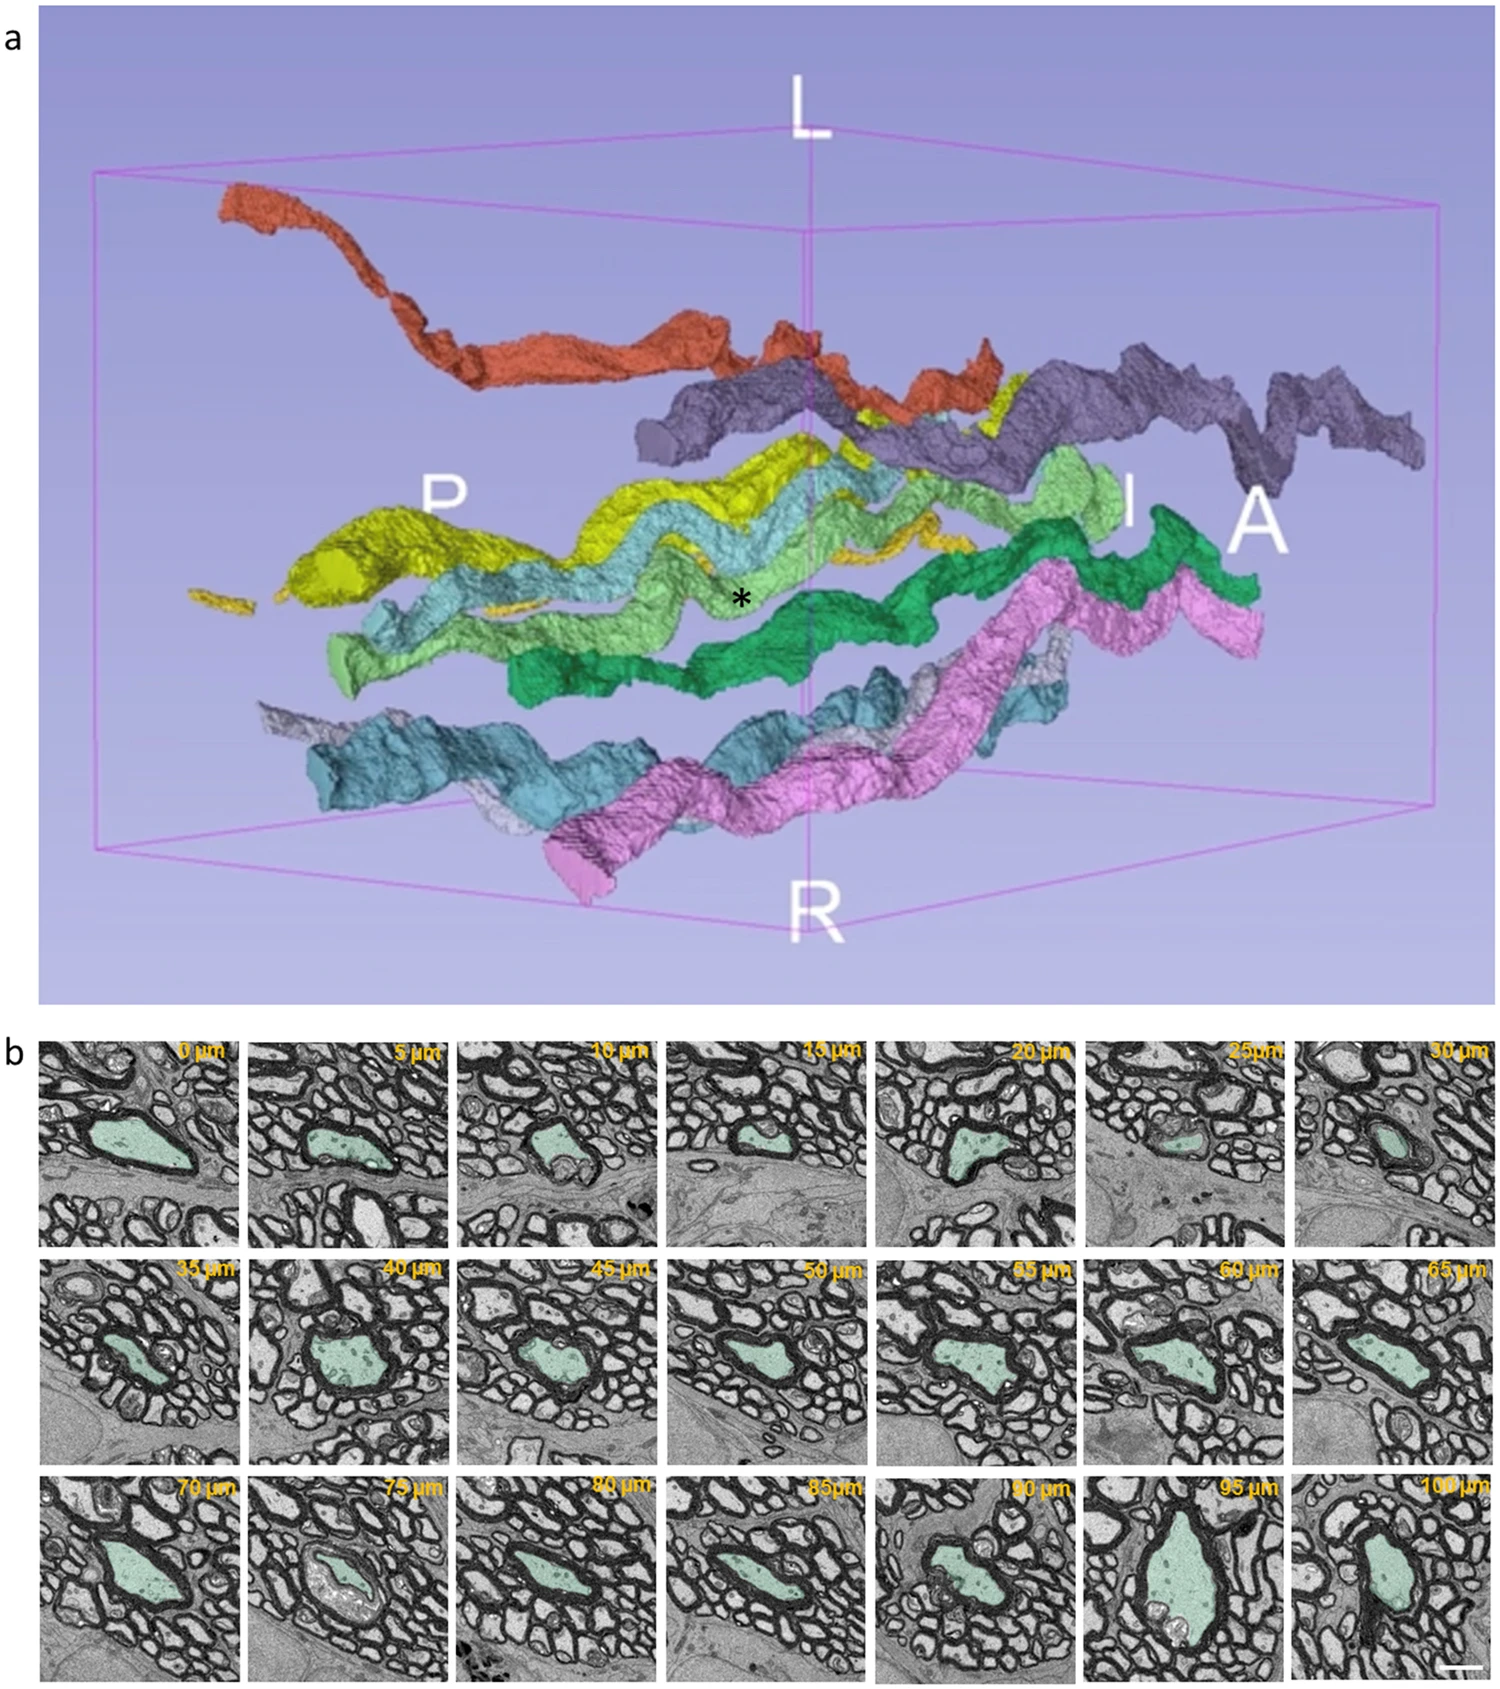
\includegraphics{gfx/neuroanatomy/nature_3d_em_optical_nerve.png}
	\caption{\todo{only show a}Three dimensional electron microscopy reveals changing axonal and myelin morphology along normal and partially injured (*, light green) optic nerves. Origin: \cite{Giacci2018} (reative Commons Attribution 4.0 International License).}
% 	\label{fig:brain_sectioning}
\end{figure}
%
% 
\begin{figure}[!t]
	\centering
	\includegraphics{gfx/neuroanatomy/magic.png}
	\caption{Magic. TPFM auto fluorescence nerve fibers. Origin: \cite{Costantini2020}.}
% 	\label{fig:brain_sectioning}
\end{figure}
% 
\section{Microscopy}
% 
Axon diameter \cite{Liewald2014}:
% 
\begin{table}[!b]
\centering
\pgfplotstabletypeset[
thesisTableStyle,
font=\footnotesize,
col sep=comma,
columns/Name/.style={string type},
columns/Mean/.style={fixed zerofill},
columns/SD/.style={fixed zerofill},
columns/Median/.style={fixed zerofill},
columns/Max/.style={fixed zerofill},
columns/Min/.style={fixed zerofill},
columns/n/.style={dec sep align},
rowbf={1},rowbf={8},rowbf={19},
rowem={2},rowem={5},
rowem={9},rowem={12},rowem={15},
rowem={20},rowem={23},rowem={26},
]{data/axon_distribution.csv}
\caption{axon diameter distribution of the human brain in \si{\micro\meter} \cite{Liewald2014}}
\end{table}
axon = 0.5-1.0 diameter (most frequent
thickness of myelin mean = 0.09, median 0.08
-> g-ratio 0.9 (electron microscop, upper boundry)
% 
g-ratio
\cite{Cercignani2017} -> 0.65-0.8 mrt, healty male and female different age, different regions\\
\cite{FitzGibbon2013} -> 0.58-0.84 (Retina), electron microscopy
% 
\begin{figure}[!t]
	\centering
	\tikzset{external/export next=false}
	\begin{tikzpicture}[]   
     \node[inner sep=0pt, anchor = south west] (fig) at (0,0)
       {\includegraphics[width=\textwidth]{gfx/neuroanatomy/NeuralNet-BrainAtlasDotOrg.png}};
    %  \draw[magenta, thick] (0,0) grid (13,10);
    %  \draw[<-, yellow, ultra thick] (7.75,6.25) -- ++ (30:1.42);
     \draw[yellow, ultra thick] (7.65,6.15) ellipse (1 and 0.5);
    %  \draw[<-, cyan, ultra thick] (10,4.5) -- ++ (30:1.42);
     \draw[cyan, ultra thick] (10,4.5) ellipse (2 and 1);
     \draw[white, ultra thick] (0.5,0.5) -- ++ (0:1) node[pos=0.5, above] {\small $\SI[math-rm=\mathbf,math-micro=\mathbf{\muup}]{0}{\micro\meter}$};
    \end{tikzpicture}
% 	\includegraphics[width=\textwidth]{gfx/neuroanatomy/NeuralNet-BrainAtlasDotOrg.png}
	\caption{Myelin Staining. human thalamus, sagital section. \textcolor{yellow}{yellow}: nerve fiber bundles. \textcolor{cyan}{cyan}: "neural net"}
% 	\label{fig:brain_sectioning}
\end{figure}